%!Mode:: "TeX:UTF-8"
\documentclass[a4paper,11pt,UTF8]{ctexart}

\usepackage{indentfirst} %缩进
\usepackage{xeCJK}    %使用系统字体
\usepackage{fancyhdr} %自定义页眉页脚
\pagestyle{empty}                   %不设置页眉页脚
\usepackage{amsmath, amsthm, amssymb, amsfonts} %数学公式
\usepackage[a4paper,left=3cm,right=3cm,top=3cm,bottom=3cm]{geometry}
%\usepackage[tmargin=1in,bmargin=1in,lmargin=1.25in,rmargin=1.25in]{geometry}.
\usepackage{booktabs} %插入表格
\usepackage[section]{placeins} %避免浮动
\usepackage{listings} %插入代码
\usepackage{ctex}     %中文宏包
\usepackage[svgnames, table]{xcolor} %彩色表格
\usepackage{algorithm}          %伪代码
\usepackage{algorithmicx}
\usepackage{algpseudocode}
\usepackage{algorithm,algpseudocode,float}
\usepackage{lipsum}
\usepackage{enumitem}           %调整列举环境
\usepackage{url}
\usepackage{fontspec,xunicode}
\defaultfontfeatures{Mapping=tex-text} %如果没有它,会有一些 tex 特殊字符无法正常使用,比如连字符。

\usepackage{graphicx}
\graphicspath{{imgs/}}

%%%%%%%%%%%%%%%%%%%%%%%%%%%%%%%%%%%%%%%%%%%%%%%%%%%%%%%%%%%%%%%%
% 缩进及行间距
%%%%%%%%%%%%%%%%%%%%%%%%%%%%%%%%%%%%%%%%%%%%%%%%%%%%%%%%%%%%%%%%
\setlength{\parindent}{22pt} %重新定义缩进长度
\setlength{\baselineskip}{20pt}  %定义行间距
%\renewcommand{\baselinestretch}{1.1} %定义行间距

%%%%%%%%%%%%%%%%%%%%%%%%%%%%%%%%%%%%%%%%%%%%%%%%%%%%%%%%%%%%%%%%
% 列表设置
%%%%%%%%%%%%%%%%%%%%%%%%%%%%%%%%%%%%%%%%%%%%%%%%%%%%%%%%%%%%%%%%
\setenumerate{fullwidth,itemindent=\parindent,listparindent=\parindent,itemsep=0ex,partopsep=0pt,parsep=0ex}
\setenumerate[2]{label=\alph*),leftmargin=1.5em}  %二级item设置
\setitemize{itemindent=38pt,leftmargin=0pt,itemsep=-0.4ex,listparindent=26pt,partopsep=0pt,parsep=0.5ex,topsep=-0.25ex}
\setdescription{itemindent=38pt,leftmargin=0pt,itemsep=-0.4ex,listparindent=26pt,partopsep=0pt,parsep=0.5ex,topsep=-0.25ex}

%%%%%%%%%%%%%%%%%%%%%%%%%%%%%%%%%%%%%%%%%%%%%%%%%%%%%%%%%%%%%%%%
% 图的标题行间距设置
%%%%%%%%%%%%%%%%%%%%%%%%%%%%%%%%%%%%%%%%%%%%%%%%%%%%%%%%%%%%%%%%
\newcommand{\bottomcaption}{%
\setlength{\abovecaptionskip}{6pt}%
\setlength{\belowcaptionskip}{6pt}%
\caption}


%%%%%%%%%%%%%%%%%%%%%%%%%%%%%%%%%%%%%%%%%%%%%%%%%%%%%%%%%%%%%%%%
% 字体定义
%%%%%%%%%%%%%%%%%%%%%%%%%%%%%%%%%%%%%%%%%%%%%%%%%%%%%%%%%%%%%%%%
\setmainfont{Times New Roman}  %默认英文字体.serif是有衬线字体sans serif无衬线字体
\setmonofont{Consolas}
\setCJKmainfont[ItalicFont={楷体}, BoldFont={黑体}]{宋体}%衬线字体 缺省中文字体为
\setCJKsansfont{黑体}
\punctstyle{hangmobanjiao}
%-----------------------xeCJK下设置中文字体------------------------------%
\setCJKfamilyfont{song}{SimSun}                             %宋体 song
\newcommand{\song}{\CJKfamily{song}}
\setCJKfamilyfont{fs}{FangSong}                      %仿宋  fs
\newcommand{\fs}{\CJKfamily{fs}}
\setCJKfamilyfont{ktgb}{KaiTi}                      %楷体2312 ktgb
\newcommand{\ktgb}{\CJKfamily{ktgb}}
\setCJKfamilyfont{yh}{Microsoft YaHei}                    %微软雅黑 yh
\newcommand{\yh}{\CJKfamily{yh}}
\setCJKfamilyfont{hei}{SimHei}                              %黑体  hei
\newcommand{\hei}{\CJKfamily{hei}}
\setCJKfamilyfont{hwxk}{STXingkai}                                %华文行楷  hwxk
\newcommand{\hwxk}{\CJKfamily{hwxk}}
%------------------------------设置字体大小------------------------%
\newcommand{\shiyanbaogao}{\fontsize{36pt}{\baselineskip}\selectfont}
\newcommand{\chuhao}{\fontsize{42pt}{\baselineskip}\selectfont}     %初号
\newcommand{\xiaochuhao}{\fontsize{36pt}{\baselineskip}\selectfont} %小初号
\newcommand{\yihao}{\fontsize{28pt}{\baselineskip}\selectfont}      %一号
\newcommand{\erhao}{\fontsize{21pt}{\baselineskip}\selectfont}      %二号
\newcommand{\xiaoerhao}{\fontsize{18pt}{\baselineskip}\selectfont}  %小二号
\newcommand{\sanhao}{\fontsize{15.75pt}{\baselineskip}\selectfont}  %三号
\newcommand{\sihao}{\fontsize{14pt}{\baselineskip}\selectfont}       %四号
\newcommand{\xiaosihao}{\fontsize{12pt}{\baselineskip}\selectfont}  %小四号
\newcommand{\wuhao}{\fontsize{10.5pt}{\baselineskip}\selectfont}    %五号
\newcommand{\xiaowuhao}{\fontsize{9pt}{\baselineskip}\selectfont}   %小五号
\newcommand{\liuhao}{\fontsize{7.875pt}{\baselineskip}\selectfont}  %六号
\newcommand{\qihao}{\fontsize{5.25pt}{\baselineskip}\selectfont}    %七号

%%%%%%%%%%%%%%%%%%%%%%%%%%%%%%%%%%%%%%%%%%%%%%%%%%%%%%%%%%%%%%%%
% 图题字体大小相同
%%%%%%%%%%%%%%%%%%%%%%%%%%%%%%%%%%%%%%%%%%%%%%%%%%%%%%%%%%%%%%%%
\usepackage{caption}
\captionsetup{font={footnotesize}}   % footnotesize = 9pt
\captionsetup[lstlisting]{font={footnotesize}}

%%%%%%%%%%%%%%%%%%%%%%%%%%%%%%%%%%%%%%%%%%%%%%%%%%%%%%%%%%%%%%%%
% 重定义枚举编号为 1),2)...
%%%%%%%%%%%%%%%%%%%%%%%%%%%%%%%%%%%%%%%%%%%%%%%%%%%%%%%%%%%%%%%%
\renewcommand{\labelenumi}{\theenumi)}


%%%%%%%%%%%%%%%%%%%%%%%%%%%%%%%%%%%%%%%%%%%%%%%%%%%%%%%%%%%%%%%%
% 重定义section标题
%%%%%%%%%%%%%%%%%%%%%%%%%%%%%%%%%%%%%%%%%%%%%%%%%%%%%%%%%%%%%%%%
\CTEXsetup[format={\sihao\CJKfamily{zhhei}\zihao{4}},number={\chinese{section}},name={,、~},aftername={},indent={0pt},beforeskip={6pt},afterskip={6pt},format+={\flushleft}]{section}
\CTEXsetup[format={\Large\bfseries\CJKfamily{zhkai}\zihao{5}},name={(,)},number={\chinese{subsection}},aftername={},indent={22pt},beforeskip={14pt},afterskip={2pt}]{subsection}
\CTEXsetup[number={\chinese{section}},name={附录, ~~ }]{appendix}



%%%%%%%%%%%%%%%%%%%%%%%%%%%%%%%%%%%%%%%%%%%%%%%%%%%%%%%%%%%%%%%%
% 标题名称中文化
%%%%%%%%%%%%%%%%%%%%%%%%%%%%%%%%%%%%%%%%%%%%%%%%%%%%%%%%%%%%%%%%
\renewcommand\figurename{\hei 图}
\renewcommand\tablename{\hei 表}
\renewcommand\lstlistingname{\hei 代码}
\renewcommand{\algorithmicrequire}{\textbf{输入:}}
\renewcommand{\algorithmicensure}{\textbf{输出:}}
\newtheorem{define}{定义}

%%%%%%%%%%%%%%%%%%%%%%%%%%%%%%%%%%%%%%%%%%%%%%%%%%%%%%%%%%%%%%%%
% 代码设置
%%%%%%%%%%%%%%%%%%%%%%%%%%%%%%%%%%%%%%%%%%%%%%%%%%%%%%%%%%%%%%%%
\lstset{
 columns=fixed,
 numbers=left,                                        % 在左侧显示行号
 numberstyle=\tiny\color{gray},                       % 设定行号格式
 frame=single,                                        % 单线背景边框
 breaklines=true,                                     % 设定LaTeX对过长的代码行进行自动换行
 keywordstyle=\color[RGB]{40,40,255},                 % 设定关键字颜色
 numberstyle=\footnotesize\color{darkgray},
 commentstyle=\it\color[RGB]{0,96,96},                % 设置代码注释的格式
 stringstyle=\rmfamily\slshape\color[RGB]{128,0,0},   % 设置字符串格式
 showstringspaces=false,                              % 不显示字符串中的空格
 language=java,                                        % 设置语言
 basicstyle=\linespread{1.0}\xiaowuhao\ttfamily,                      % 字体字号
 %lineskip=10pt,
 %baselinestretch=1,
}

%%%%%%%%%%%%%%%%%%%%%%%%%%%%%%%%%%%%%%%%%%%%%%%%%%%%%%%%%%%%%%%%
% 伪代码分页
%%%%%%%%%%%%%%%%%%%%%%%%%%%%%%%%%%%%%%%%%%%%%%%%%%%%%%%%%%%%%%%%
\makeatletter
\renewcommand{\ALG@name}{算法}
\newenvironment{breakablealgorithm}
  {% \begin{breakablealgorithm}
   \begin{center}
     \refstepcounter{algorithm}% New algorithm
     \hrule height.8pt depth0pt \kern2pt% \@fs@pre for \@fs@ruled
     \renewcommand{\caption}[2][\relax]{% Make a new \caption
       {\raggedright\textbf{\ALG@name~\thealgorithm} ##2\par}%
       \ifx\relax##1\relax % #1 is \relax
         \addcontentsline{loa}{algorithm}{\protect\numberline{\thealgorithm}##2}%
       \else % #1 is not \relax
         \addcontentsline{loa}{algorithm}{\protect\numberline{\thealgorithm}##1}%
       \fi
       \kern2pt\hrule\kern2pt
     }
  }{% \end{breakablealgorithm}
     \kern2pt\hrule\relax% \@fs@post for \@fs@ruled
   \end{center}
  }
\makeatother



\begin{document}
\xiaosihao\song

\begin{titlepage}
\center{\yihao{\hwxk{武汉大学国家网络安全学院}}}
\vspace{6cm}
\center{\shiyanbaogao{\ktgb{信~息~隐~藏~实~验~报~告}}}
\vspace{4cm}

\begin{center}
\begin{large}
\begin{tabular}{rc}
\xiaoerhao{\hei{学\qquad 号}}& \hspace{1.7cm}\xiaoerhao{\hei{2021302181156\hspace{1.7cm}}} \\
\cline{2-2}\\
\xiaoerhao{\hei{姓\qquad 名}}& \xiaoerhao{\hei{赵伯俣}}\\
\cline{2-2}\\
\xiaoerhao{\hei{实验名称}}& \xiaoerhao{\hei{基本图像信息隐藏方法实践}}\\
\cline{2-2}\\
\xiaoerhao{\hei{指导教师}}& \xiaoerhao{\hei{任延珍}}\\
\cline{2-2}
\end{tabular}
\end{large}
\end{center}
\vfill \hfill
\end{titlepage}
\clearpage

% \centerline{\\[10pt]\erhao{\fs{武 ~汉 ~ 大~ 学}}}
% \centerline{\\[10pt]\yihao{\fs{信~息~隐~藏~实~验~报~告}}}

% \leftline{\\[10pt]\sihao{\hei{\hspace{1.5em} 学生姓名:XXX \hfill 学号:XXXX \hfill 指导教师:XXX }}}

% \leftline{\\[10pt]\sihao{\hei{\hspace{1.5em} 实验地点:新珈楼XXX \hfill }}}

% \leftline{\\[10pt]\sihao{\hei{\hspace{1.5em} 实验时间:第X周周X(X-X节) \hfill }}}



\setlength{\parskip}{6pt}  %定义段间距

\section{实验名称: 基本图像信息隐藏方法实践}
\section{实验目的:}
  {
    1.学习matlab的基本操作。\\
    \hspace*{22pt}2.实现图像的LSB隐写和隐藏信息的提取。\\
    \hspace*{22pt}3.使用两点法实现图像的DCT域隐写与隐写信息的提取。
  }

\section{实验原理:}

  \subsection{LSB隐写}
  将我们选取的像素点的最不重要位依次替换成秘密信息, 以达到信息隐秘的目的。
  嵌入过程包括选择一个图像载体像素点的子集, 然后在子集上执行替换操作像素 
  把整个图像的 LSB 与秘密信息 mi 进行交换(mi是秘密信息的二进制表示) 。一个替
  换系统也可以修改载体图像像素点的多个比特。\par
  在本次实验中选取一张图片提取出其图像二进制编码的最后一位替换为秘密信息进行信息隐藏。
  原理图如下所示。

  \begin{figure}[!htbp]
  \centering
  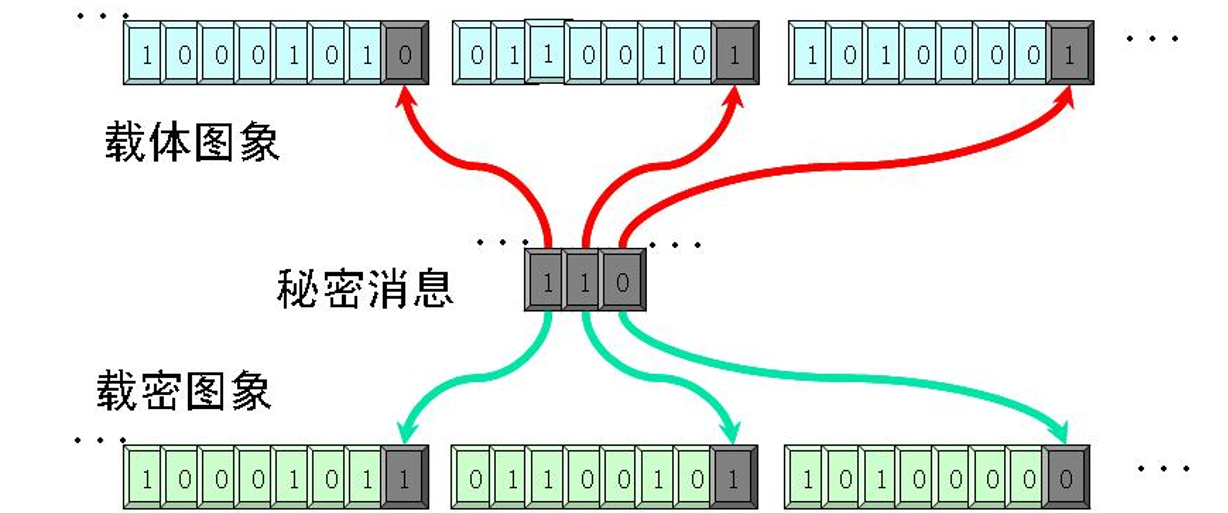
\includegraphics[width=\textwidth]{LSB.png}
  \bottomcaption{\xiaowuhao{LSB隐写原理}}
  \end{figure}

  \subsection{DCT变换对图像进行压缩}
    在DCT变换中使用如下数学公式对图像进行离散余弦变换,在压缩过后的图像中低频部分往往保存了图像的大部分信息,
    高频部分保存的信息往往较少,因此可以通过删除图像的部分高频信息的方式对图像的大小进行压缩但不较大幅度改变图像质量。
    \begin{figure}[!htbp]
    \centering
    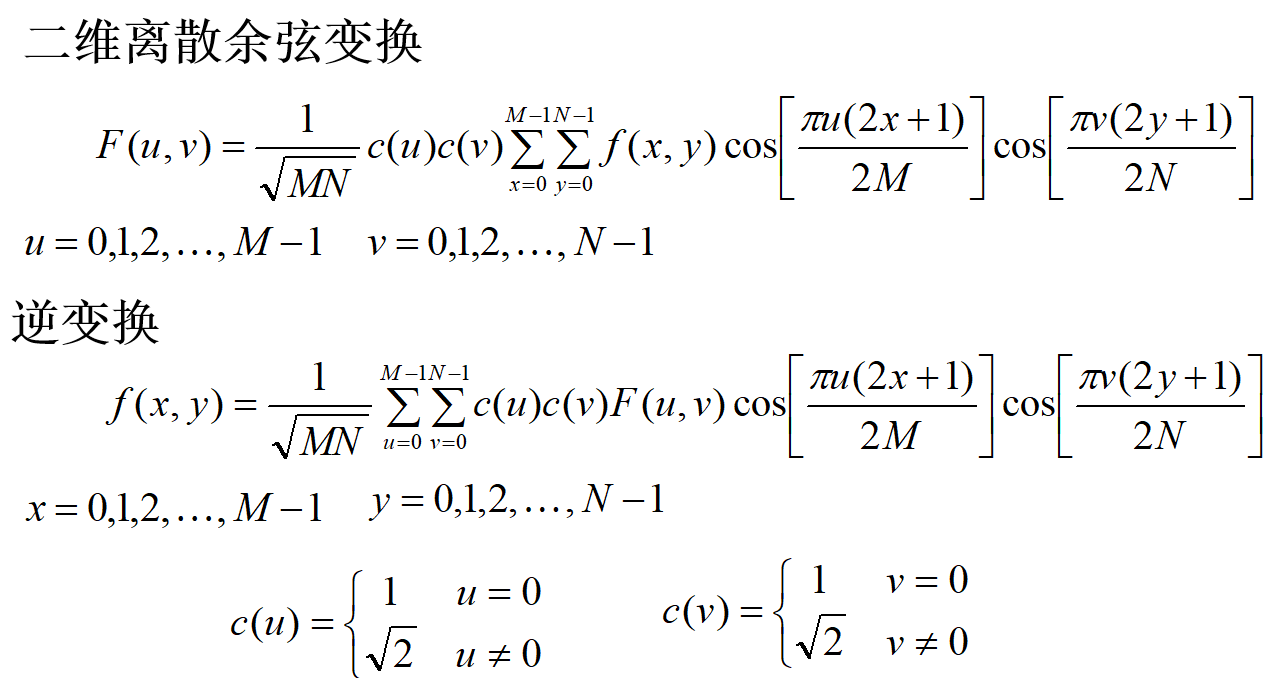
\includegraphics[width=\textwidth]{DCT_math.png}
    \bottomcaption{\xiaowuhao{DCT压缩原理}}
    \end{figure}

  \subsection{DCT域隐写}
  对一幅图像进行离散余弦变换后,许多有关图像的重要可视信息都集中在DCT变换的一小部分系数中。可以将秘密信息隐藏在变换后的图像之中。
  在本次实验中采用两点法进行信息的隐藏,选取两个点,利用载体中两个特定数的相对大小来代表隐藏的信息。
  \begin{figure}[!htbp]
  \centering
  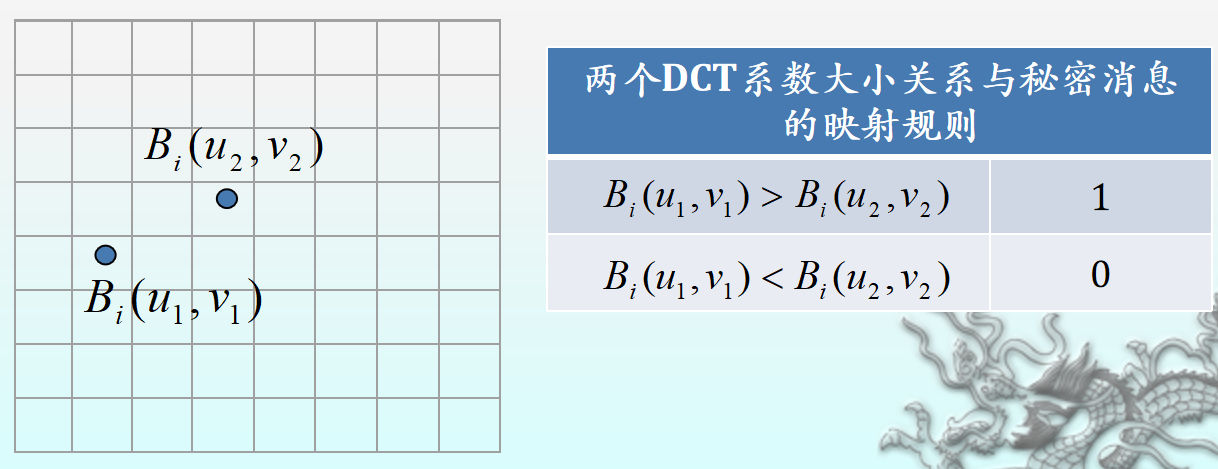
\includegraphics[width=\textwidth]{DCT.png}
  \bottomcaption{\xiaowuhao{DCT隐写原理}}
  \end{figure}


\section{实验内容:}

  \subsection{实验一:LSB隐写}
    LSB信息隐藏的代码如下所示
    \lstinputlisting[caption={LSB隐写代码},captionpos=b]{D:/matlab_codes/randlsbhide/randlsbhide.m}
    LSB信息提取的代码如下图所示
    \lstinputlisting[caption={LSB信息提取代码},captionpos=b]{D:/matlab_codes/randlsbget/randlsbget.m}
    调用的随机间隔函数选取像素点代码如下图所示
    \lstinputlisting[caption={随机间隔函数代码},captionpos=b]{D:/matlab_codes/randlsbhide/randinterval.m}
      
  \subsection{实验二:DCT变换对图像进行压缩}
    DCT变换对图像进行压缩的代码如下所示
    \lstinputlisting[caption={DCT变换图像压缩代码},captionpos=b]{D:/matlab_codes/dct_change/dctcom.m}

  \subsection{实验三:DCT域隐写}
    在DCT域进行隐写的代码如下所示
    \lstinputlisting[caption={DCT域隐写与信息提取算法},captionpos=b]{D:/matlab_codes/dcthide/dcthide2.m}

    对误码率进行分析的代码如下图所示
    \lstinputlisting[caption={DCT域隐写误码率分析函数},captionpos=b]{D:/matlab_codes/dcthide/draw.m}

\section{实验环境:}
  1.win11操作系统\par
  2.MATLAB R2022a

\section{实验步骤:}

  \subsection{实验一:LSB隐写}
    \subsubsection{设计随机取点的算法,随机选取像素点嵌入秘密信息}
      首先先将保存有秘密信息的文本文件转换成二进制文件存入数组msg中,并将其长度保存在变量len\_total中。
      然后调用随机间隔函数使其按照提供的密钥选取一系列的随机点坐标,然后针对密文的每一个字符msg(p,1),
      选定其要保存的像素块ste\_cover(row(i),col(i)),将该像素块的二进制最后一位清零然后加上msg(p,1),
      将所有的密文隐藏入图像中之后将图片输出为scover.bmp的形式。

    \subsubsection{提取秘密信息}
      输入隐藏有密文的图像和密文长度之后提取图像LSB的最后一位二进制信息,逐个随机点坐标进行提取即可
      提取到密文长度数量的二进制信息,将信息输出成为一个保存有秘密信息的txt文件。

    \subsubsection{画出随机位置}
      编写compare函数求经过LSB隐写后的文件与原图像的差值,将差值作为图像绘制出来就能够得到由密钥key生成的所有的随机位置。
      compare比较函数的代码如下所示。
      \lstinputlisting[caption={绘制所有随机位置的函数代码},captionpos=b]{D:/matlab_codes/randlsbhide/compare.m}

    \subsubsection{对比隐写前后图像直方图,分析LSB隐写导致的值对效应}
      编写绘制加密前后图像的直方图的函数对图像的值对效应进行比较,绘制图像直方图的函数如下所示。
      \lstinputlisting[caption={绘制图像直方图函数代码},captionpos=b]{D:/matlab_codes/randlsbhide/draw.m}

 
  \subsection{实验二:DCT变换对图像进行压缩}
    \subsubsection{图像分块}
      首先将图像进行分块处理,在本次实验中,将整个图像分成了8*8大小的块分别进行处理
    \subsubsection{删除部分DCT系数}
      设置矩阵mask对DCT系数进行量化,将矩阵的左上角部分置为1,其余部分置为0,即保留原图像的低频部分,删除掉图像的高频部分
    \subsubsection{逆DCT变换}
      将经过DCT变换后逆DCT变换的块拼到一起后形成操作后的图像,将原图和操作后的图像进行输出比较。

  \subsection{实验三:DCT域隐写}
    \subsubsection{图像预处理}
      提取RGB图像的红色位所有数据作为信息隐藏的载体,以满足对于所有的信息载体都能够处理的要求。
      保留原图像的其他位的数据,
    \subsubsection{t图像分块后做二维DCT变换}
      将图像进行分块后得到8*8的分块,设计量化矩阵,将矩阵的左上角数值设置得尽可能小,右下角数值尽可能大,
      以实现尽可能多的保存图像的低频数据对图像实行二维DCT变换。
    \subsubsection{隐藏信息}
      对于第x个bit的信息,如果要隐藏的信息为1,则将C(i+u(1)-1,j+u(2)-1)设置为大于C(i+v(1)-1,j+v(2)-1),
      其中C(i+u(1)-1,j+u(2)-1)和C(i+v(1)-1,j+v(2)-1)表示在该分块下约定好的两块的位置。
    \subsubsection{逆DCT变换,还原图像}
      将隐藏好信息的块合并到一起形成完整的原图红色色域的图像,将原图其他两个色域的图像与其叠加形成三维RGB图像,
      将原图和经过处理的图像进行输出和保存操作。

\newpage
\section{实验结果与分析:}
  \subsection{实验一:LSB隐写}
    \begin{itemize}
      \item 隐写结果
        LSB隐写之后的图片和原图的对比如下图所示,通过肉眼比较几乎不能够看出其中的差异。
        \begin{figure}[!htbp]
        \centering
        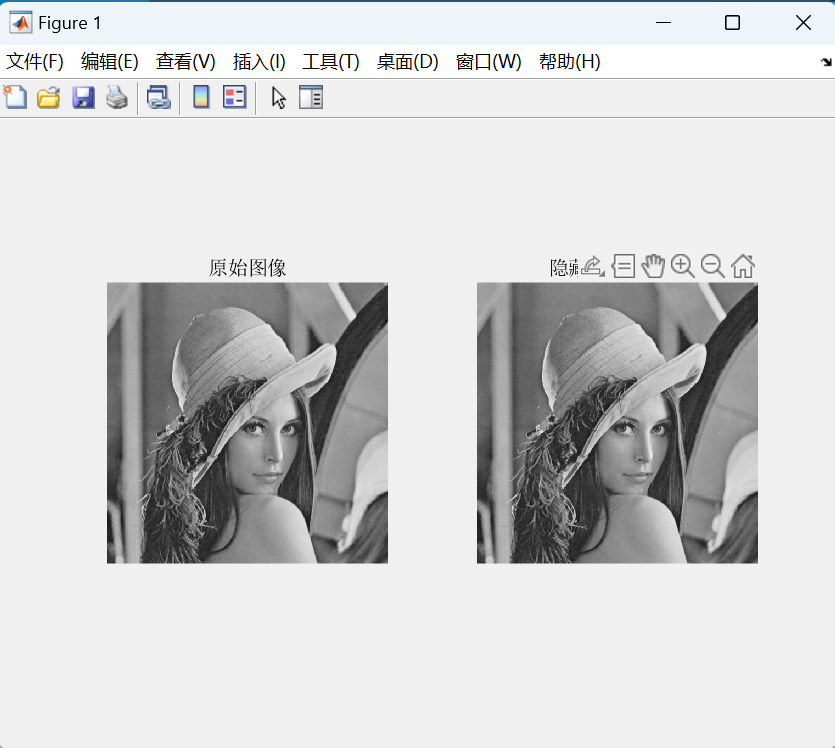
\includegraphics[width=\textwidth]{LSB_result1.png}
        \bottomcaption{\xiaowuhao{LSB隐写前后图像}}
        \end{figure}
\newpage
      \item 画出随机位置的结果
        运行比较函数比较原图和LSB隐写之后的图片结果如下图所示,可以看到在图像中存在一些较为明显的
        白色像素点和黑色像素点。
        \begin{figure}[!htbp]
        \centering
        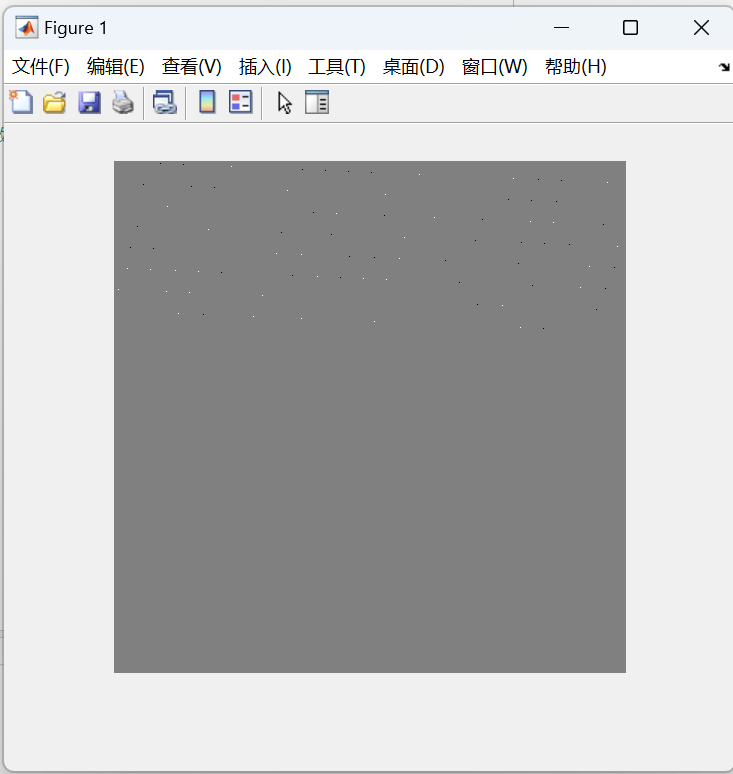
\includegraphics[width=\textwidth]{LSB_compare_result.png}
        \bottomcaption{\xiaowuhao{生成的所有的随机位置}}
        \end{figure}
    
\newpage
      \item 画出隐写前后的图像直方图,分析值对效应
        在运行函数draw之后生成原图和隐写后图像的直方图,观察两张图片的值对效应\par
        \begin{figure}[!htbp]
        \centering
        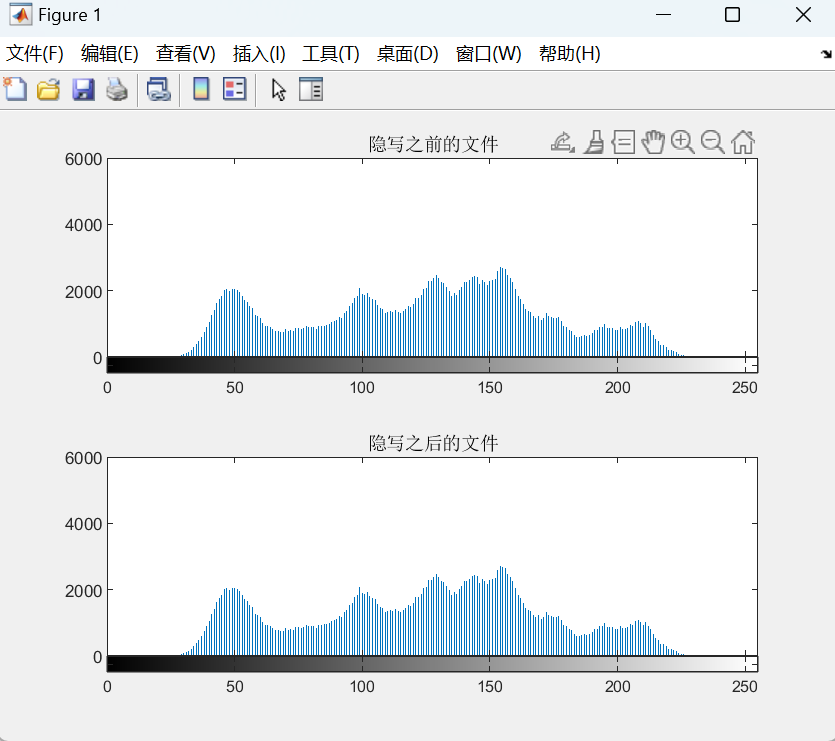
\includegraphics[width=\textwidth]{LSB_draw.png}
        \bottomcaption{\xiaowuhao{隐写前后图像直方图}}
        \end{figure}
        通过肉眼观察很难发现两个直方图中的值对效应,所以在代码中对每一个图像的像素值进行了统计,统计方法为
        将像素值为i的像素个数与像素值为i+1的像素值做差取绝对值后求整个图像的总和。对隐写前后的统计结果分析如下表所示\par
        \begin{table}[!h!tbp]
          \caption{隐写前后图像值对效应统计}\label{tab1}
            \centering
          \begin{tabular*}{0.75\textwidth}{@{\extracolsep{\fill}}lcc}
              \toprule
              图像          &值对差值总和                \\
              \midrule
              原图              &15288         \\
              隐写后图像        &15282        \\
              \bottomrule
          \end{tabular*}
        \end{table}
        由此可见隐写后的图像值对插值总和相对较低,具有较强的值对效应
    \end{itemize}

  \subsection{实验二:DCT变换对图像进行压缩}
    \begin{itemize}
      \item 图像压缩前后的结果如下图所示\par
        \begin{figure}[!htbp]
        \centering
        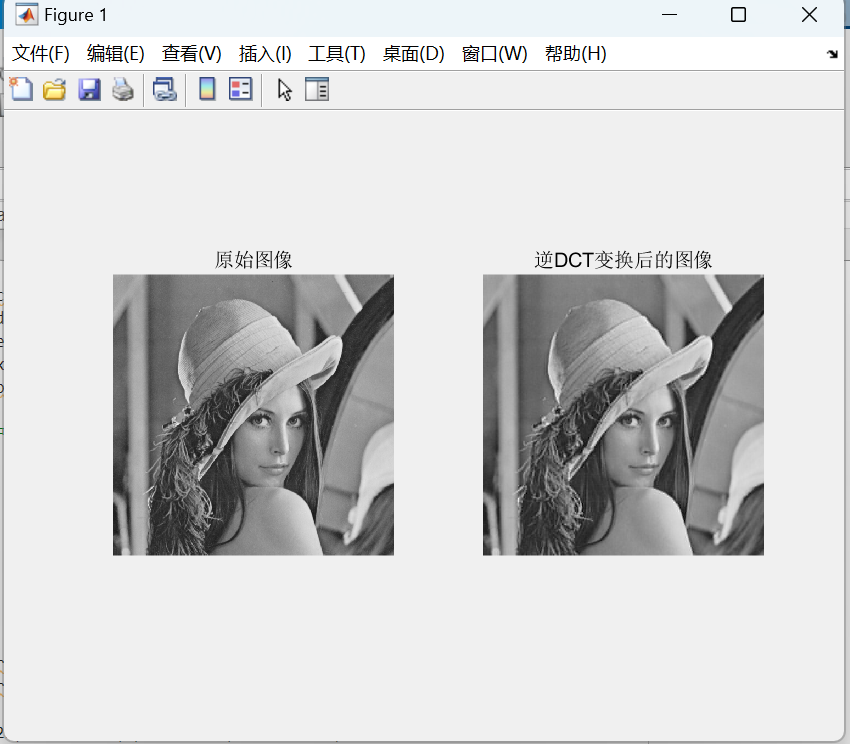
\includegraphics[width=\textwidth]{DCT_change_result.png}
        \bottomcaption{\xiaowuhao{DCT变换前后图像对比}}
        \end{figure}
      \item 结果分析\par
        通过对DCT压缩前后的图像的视觉质量进行分析可以看出即使删除了图像DCT变换后的高频系数,
        在肉眼观察上仍然不能够发现两张图片的差异。
    \end{itemize}
  
\newpage
  \subsection{实验三:DCT域隐写}
  \begin{itemize}
    \item DCT域隐写结果\par
      DCT隐写后的图像和原图如下图所示,经过肉眼观察并不能够发现其中存在的变化。\par
      \begin{figure}[!htbp]
      \centering
      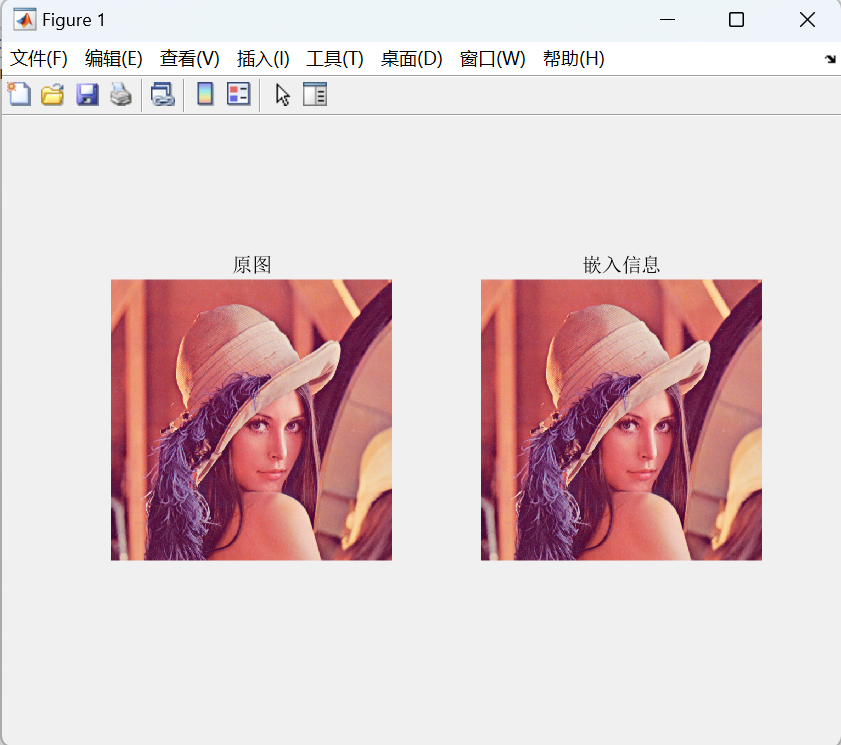
\includegraphics[width=\textwidth]{DCThide_result1.png}
      \bottomcaption{\xiaowuhao{DCT隐写前后图像}}
      \end{figure}
\newpage
    \item DCT数据提取结果\par
      DCT数据提取结果与原始秘密信息的对比如下图所示。
        \begin{figure}[!htbp]
        \centering
        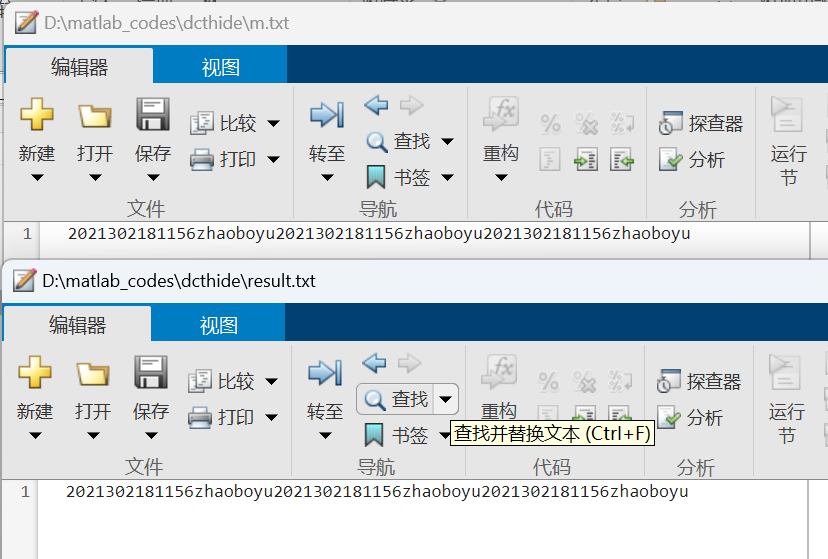
\includegraphics[width=\textwidth]{DCTget_result.png}
        \bottomcaption{\xiaowuhao{DCT提取结果}}
        \end{figure}
      
    \item 分析健壮参数和鲁棒性
        运行健壮参数和鲁棒性分析代码后的结果如下图所示:
        \begin{table}[!h!tbp]
          \caption{分析健壮参数和鲁棒性}\label{tab2}
            \centering
          \begin{tabular*}{0.75\textwidth}{@{\extracolsep{\fill}}lcc}
              \toprule
              健壮参数          &误码个数       &误码率                \\
              \midrule
              0.1                 &0           &0.00\%               \\
              0.01                &0           &0.00\%           \\
              0.001               &0           &0.00\%            \\
              0.0005              &2           &0.40\%          \\
              0.0004              &10          &1.98\%            \\
              0.0001              &59          &11.70\%          \\
              0.00001             &75          &14.88\%         \\
              \bottomrule			
          \end{tabular*}
        \end{table}\par
        经过上表的结果可以看出健壮参数的值越小,提取信息的误码率就越高,图像的鲁棒性就越差。
  \end{itemize}

\section{总结及心得体会:}
    1.在分析DCT隐写的鲁棒性时仅仅列出了实验表格,没有将实验数据化成直方图的形式。\par
    2.实验中仅对一张Lena图片进行了操作,没有针对更多其他格式其它类型的图片进行操作。\par
    3.实验代码运行的过程中没能处理好函数间的关系,导致写出的函数可观性较差,运行较为复杂,不能直接运行
\vspace{4cm}
\begin{flushright}
\begin{tabular}{lc}
\end{tabular}
\end{flushright}

\end{document}
